\chapter{MLOps - Development and Operations Integrated}


%================================================================================
%
%================================================================================
\section{DevOps and MLOps – Foundations and Motivation}

We would like to explore the approach to software development known as DevOps and MLOps (for machine learning). It is widely used these days, and good to understand and adapt to our development of both AI techniques and traditional forecasting methods in weather, climate and environment. 

%--------------------------------------------------------------------------------
%
%--------------------------------------------------------------------------------
\subsection{What is DevOps?}
% Principles: collaboration, automation, quality assurance

DevOps is a modern approach to software engineering that fosters close collaboration between development (``Dev'') and operations (``Ops'') teams. The primary goal is to shorten the development lifecycle and increase the frequency and reliability of software releases.

\begin{figure}[ht]
\centering
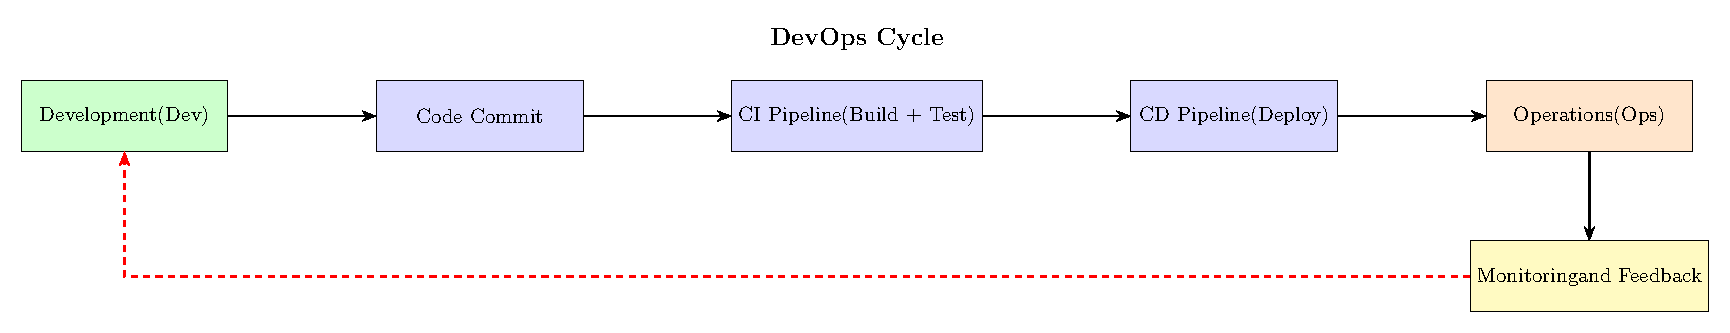
\includegraphics[width=0.9\textwidth]{images/devops1.pdf}
\caption{The DevOps cycle integrates development and operations through automation and feedback loops. This enhances deployment speed and system reliability.}
\end{figure}


Traditional development and operations workflows were often separated by organizational boundaries: developers wrote the code, and operations teams deployed and maintained it. This led to communication gaps, deployment delays, and quality issues. DevOps bridges this gap through shared responsibilities, continuous feedback loops, and a high degree of automation.

\paragraph{Core Principles of DevOps:}
\begin{itemize}
	\item \textbf{Collaboration:} Developers, testers, and system operators work in integrated teams with shared goals and tools.
	\item \textbf{Automation:} Build, test, deployment, and infrastructure provisioning processes are automated to reduce errors and manual effort.
	\item \textbf{Continuous Integration and Deployment (CI/CD):} New code is regularly merged, tested, and deployed in automated pipelines.
	\item \textbf{Monitoring and Feedback:} Systems are continuously monitored in production, and feedback from users and metrics is used to improve quality and performance.
\end{itemize}

\paragraph{Benefits of DevOps:}
\begin{itemize}
	\item Faster and more frequent releases
	\item Higher software quality and stability
	\item Shorter time to recover from failures
	\item Better alignment with user needs and operational constraints
\end{itemize}

DevOps has become a cornerstone of agile software delivery in modern organizations and is foundational for adopting MLOps in the context of machine learning systems.

%--------------------------------------------------------------------------------
%
%--------------------------------------------------------------------------------
\subsection{What is MLOps?}
% Extension of DevOps: model handling, data, lifecycle challenges

MLOps (Machine Learning Operations) is the extension of DevOps principles to the field of machine learning. While DevOps focuses on the automation and quality assurance of software development and deployment, MLOps addresses the unique challenges involved in managing machine learning workflows, from data ingestion and model training to deployment, monitoring, and retraining.

\begin{figure}[ht]
  \centering
  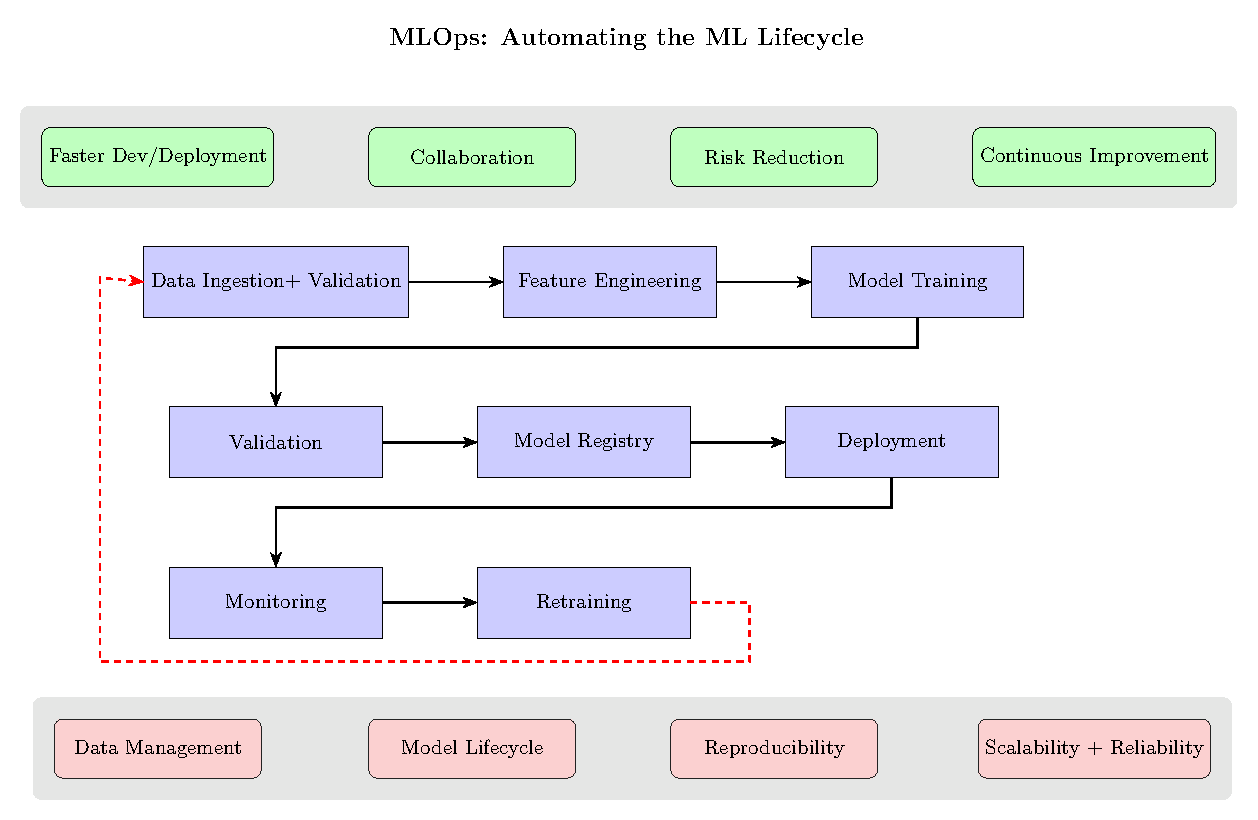
\includegraphics[width=\textwidth]{images/mlops_pipeline.pdf}
  \caption{MLOps extends DevOps by managing not only software but also data and model lifecycles. The diagram shows a typical pipeline with associated goals and challenges.}
  \label{fig:mlops-pipeline}
\end{figure}


Machine learning systems differ from traditional software in several key aspects. They are not just driven by code but also by data and model parameters. As a result, additional components and responsibilities are introduced into the development and operations lifecycle.

{\bf Key challenges addressed by MLOps.} MLOps addresses several fundamental obstacles that arise when bringing machine learning systems from research to production. These include:
{\bf Data management}, which involves tracking versions of datasets, handling preprocessing pipelines, and ensuring \textbf{clear data lineage};
{\bf model lifecycle management}, covering training, validation, deployment, monitoring, and eventual retirement of models; 
{\bf reproducibility}, which ensures that models can be retrained and redeployed under consistent conditions, accounting for randomness, hardware, and dependencies; and 
{\bf scalability and reliability}, referring to the ability of deployed models to handle increasing workloads while maintaining stable performance in dynamic environments.

{\bf Typical Components of an MLOps Pipeline.} A typical MLOps pipeline consists of several components that work together to ensure robust and automated model lifecycle management: 
\textbf{Data ingestion and validation}, where raw data is collected, checked for consistency, and validated for correctness; 
\textbf{feature engineering pipelines}, which transform and encode data into suitable formats for model training; 
\textbf{training pipelines and model validation}, which automate the training process and evaluate performance using cross-validation or test datasets; 
\textbf{model registry and version control}, where trained models are stored, versioned, and tagged for reproducibility; 
\textbf{deployment and inference services}, which provide access to models via APIs or batch processing tools; 
\textbf{monitoring and performance tracking}, to observe models in production and detect drifts or failures; and 
\textbf{automated retraining or rollback mechanisms}, which allow models to be updated or reverted without manual intervention.


{\bf Goals of MLOps.}
\begin{itemize}
	\item Increase the speed and robustness of model development and deployment
	\item Improve collaboration between data scientists, ML engineers, and IT operators
	\item Reduce operational risk by integrating testing, monitoring, and rollback strategies
	\item Enable continuous improvement of deployed models through automation
\end{itemize}

MLOps plays a critical role in bringing machine learning models into production environments in a systematic and controlled way. It ensures that models are not only developed effectively but also maintained, monitored, and updated reliably.

\begin{figure}[ht]
  \centering
  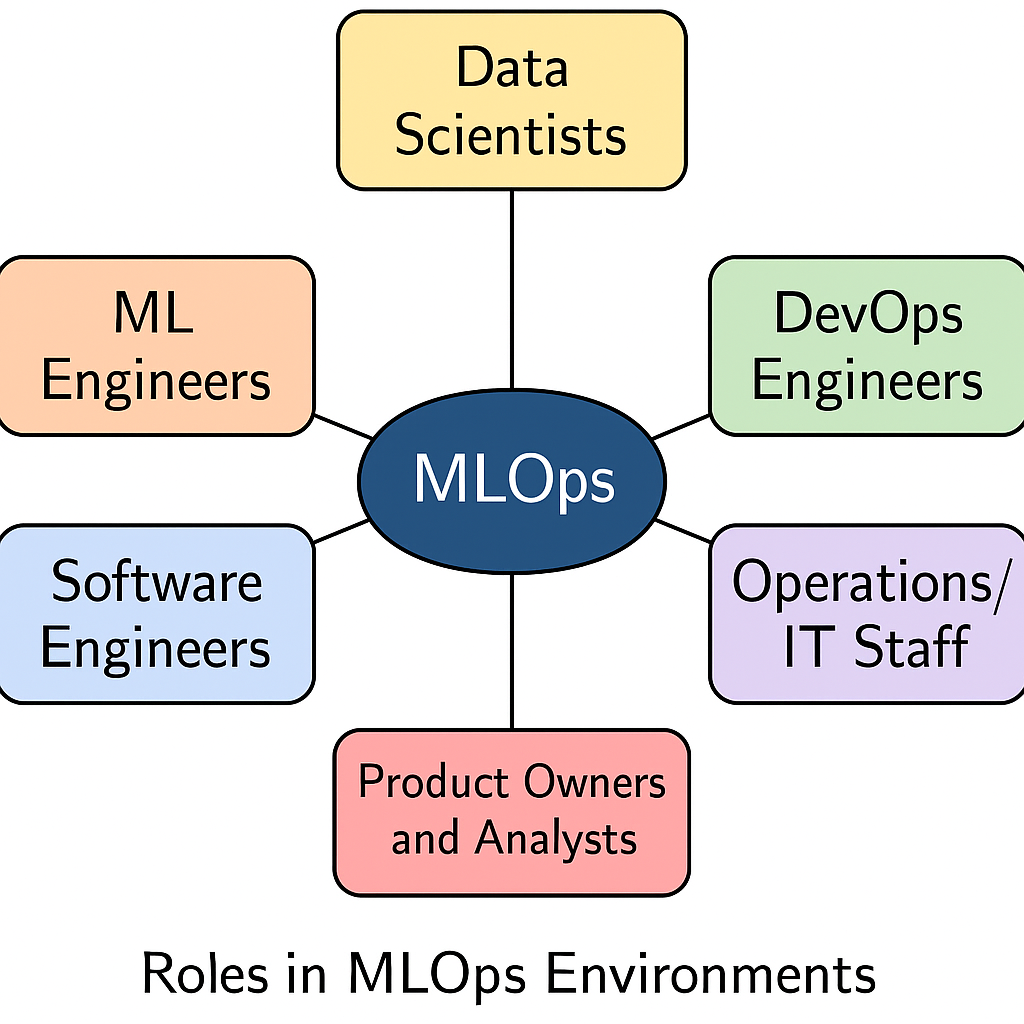
\includegraphics[width=0.6\textwidth]{images/mlops_roles.png}
  \caption{Key roles involved in MLOps environments, each contributing to the model lifecycle from experimentation to deployment and monitoring.}
  \label{fig:mlops-roles}
\end{figure}


\subsection{Roles in MLOps Environments}

Let us look at the experiences from a countless number of IT projects, putting it into a perspective of our own IT competence and experience! A lot of people realized that the successful implementation of MLOps requires collaboration across multiple roles with distinct yet complementary responsibilities. Unlike traditional software projects, ML initiatives combine software engineering with data-centric experimentation. This interdisciplinary nature brings together diverse profiles that must work in coordination throughout the model lifecycle.


\noindent
\textbf{Key roles in an MLOps team} typically include the following:

\begin{itemize}
	\item \textbf{Data Scientists:} 
	Responsible for data exploration, feature engineering, model development, and performance evaluation. They experiment with algorithms and optimize models for accuracy and generalization.
	
	\item \textbf{ML Engineers:} 
	Bridge the gap between data science and operations. They build robust training pipelines, manage model versioning, and prepare models for deployment. Often, they transform experimental code into scalable systems.
	
	\item \textbf{DevOps Engineers:} 
	Provide infrastructure, automation, and monitoring tools. They implement CI/CD pipelines, manage cloud or HPC environments, and support system reliability and scalability.
	
	\item \textbf{Software Engineers:} 
	Integrate ML components into broader applications, develop APIs and UIs, and ensure code quality, modularity, and long-term maintainability.
	
	\item \textbf{Operations and IT Staff:} 
	Maintain and secure the underlying infrastructure, including compute clusters, storage systems, networks, and access control mechanisms.

	\item \textbf{Product Owners and Analysts:} 
	Translate user needs into measurable objectives and success metrics. They guide development priorities and ensure alignment with business or scientific goals.
\end{itemize}

\noindent
\textbf{Collaboration is Essential.} Effective MLOps requires ongoing communication and tight feedback loops between these roles. Continuous integration and deployment are not just technical challenges — they are organizational. A shared-responsibility model fosters transparency, reduces misalignment, and supports iterative improvement.

In weather services and similar domains, these roles are often distributed across departments such as research, operations, and IT. This makes clear interfaces, automation, and reproducible workflows even more critical for success.

%--------------------------------------------------------------------------------
%
%--------------------------------------------------------------------------------
\subsection{Special Considerations in Weather Services}
% Differences from classical IT operations, goal setting, expectations

Weather services have traditionally operated large-scale, mission-critical systems with strict requirements for availability, reliability, and accuracy. The integration of machine learning into this domain introduces new opportunities -- but also new challenges -- that differ significantly from classical IT environments or typical business-driven ML use cases.

\begin{figure}[ht]
  \centering
  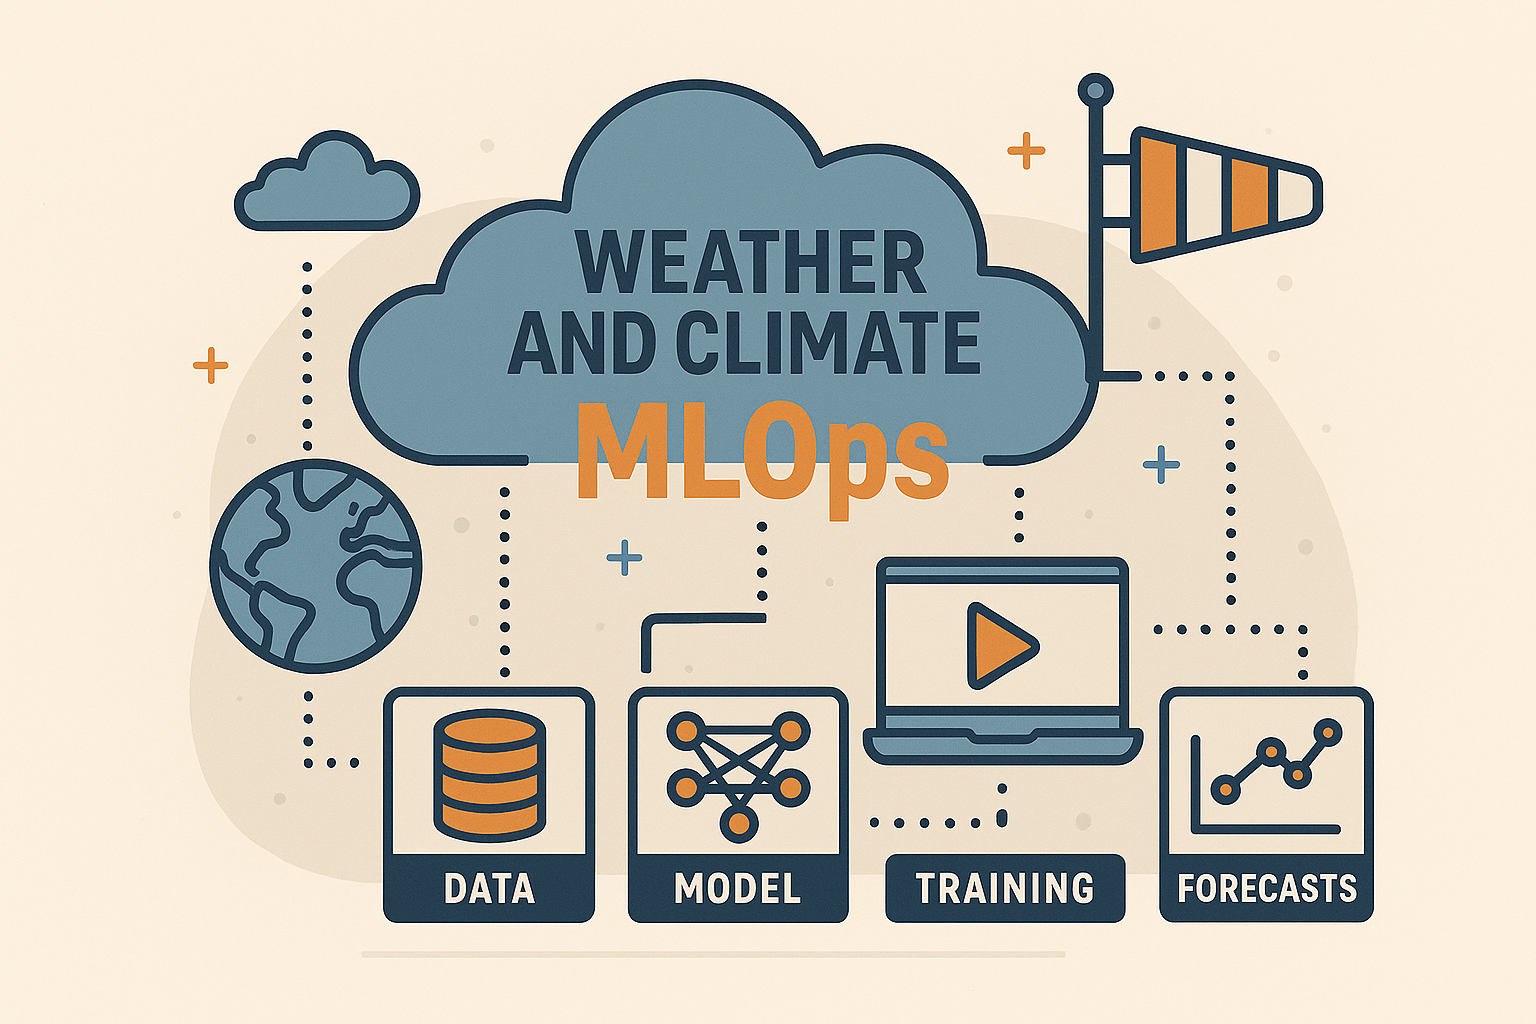
\includegraphics[width=0.7\textwidth]{images/mlops_weather.png}
  \caption{Illustration of MLOps in the context of weather and climate prediction. The pipeline integrates data ingestion, model development, training infrastructure, and forecast delivery in a cohesive operational framework.}
  \label{fig:mlops-weather}
\end{figure}


{\bf Operational constraints.} Forecasting systems must run on fixed schedules, synchronized with observation and dissemination cycles. Delays or failures can affect downstream warning systems and international data exchange.

{\bf High-performance computing (HPC) environments.} Numerical weather prediction (NWP) relies heavily on tightly optimized HPC systems. ML systems must often be integrated into these environments, which are less flexible than cloud platforms and have strict policies for software deployment.

{\bf Long-established workflows.} Many forecasting systems are built on decades of development and have been refined for performance and stability. These systems often rely on scripting tools, such as {\em BACY} and {\em NUMEX} at DWD, which already enable a partial form of DevOps by automating development and production chains.

{\bf Collaboration across departments.} Development and operations are often split across research units, IT, and forecast offices. This requires particularly clear interfaces and responsibilities when introducing MLOps components.

{\bf Data and model lifecycles.} Weather models are physically based, whereas ML models are data-driven and empirical. This demands new verification strategies, versioning mechanisms, and traceability for datasets and training pipelines.

{\bf Regulatory and public responsibility.} Forecasts often feed into civil protection and international exchange systems, meaning ML components must meet rigorous quality and documentation standards before being accepted into operations.

Machine learning in weather services is therefore not simply a technical extension -- it requires structural, procedural, and cultural adaptation. MLOps practices must be aligned with operational weather production while remaining flexible enough to support rapid development and testing.


%================================================================================
%
%================================================================================
\section{Containerization and Reproducibility}

%--------------------------------------------------------------------------------
%
%--------------------------------------------------------------------------------
\subsection{Introduction to Container Technologies}
% Docker, Singularity/Apptainer – motivations, differences, and use cases

Container technologies have become a cornerstone of modern software engineering, enabling reproducibility, portability, and modular deployment across diverse platforms. They are particularly valuable in MLOps, where complex dependencies and hardware constraints can otherwise lead to brittle or non-reproducible systems.

\begin{figure}[ht]
  \centering
  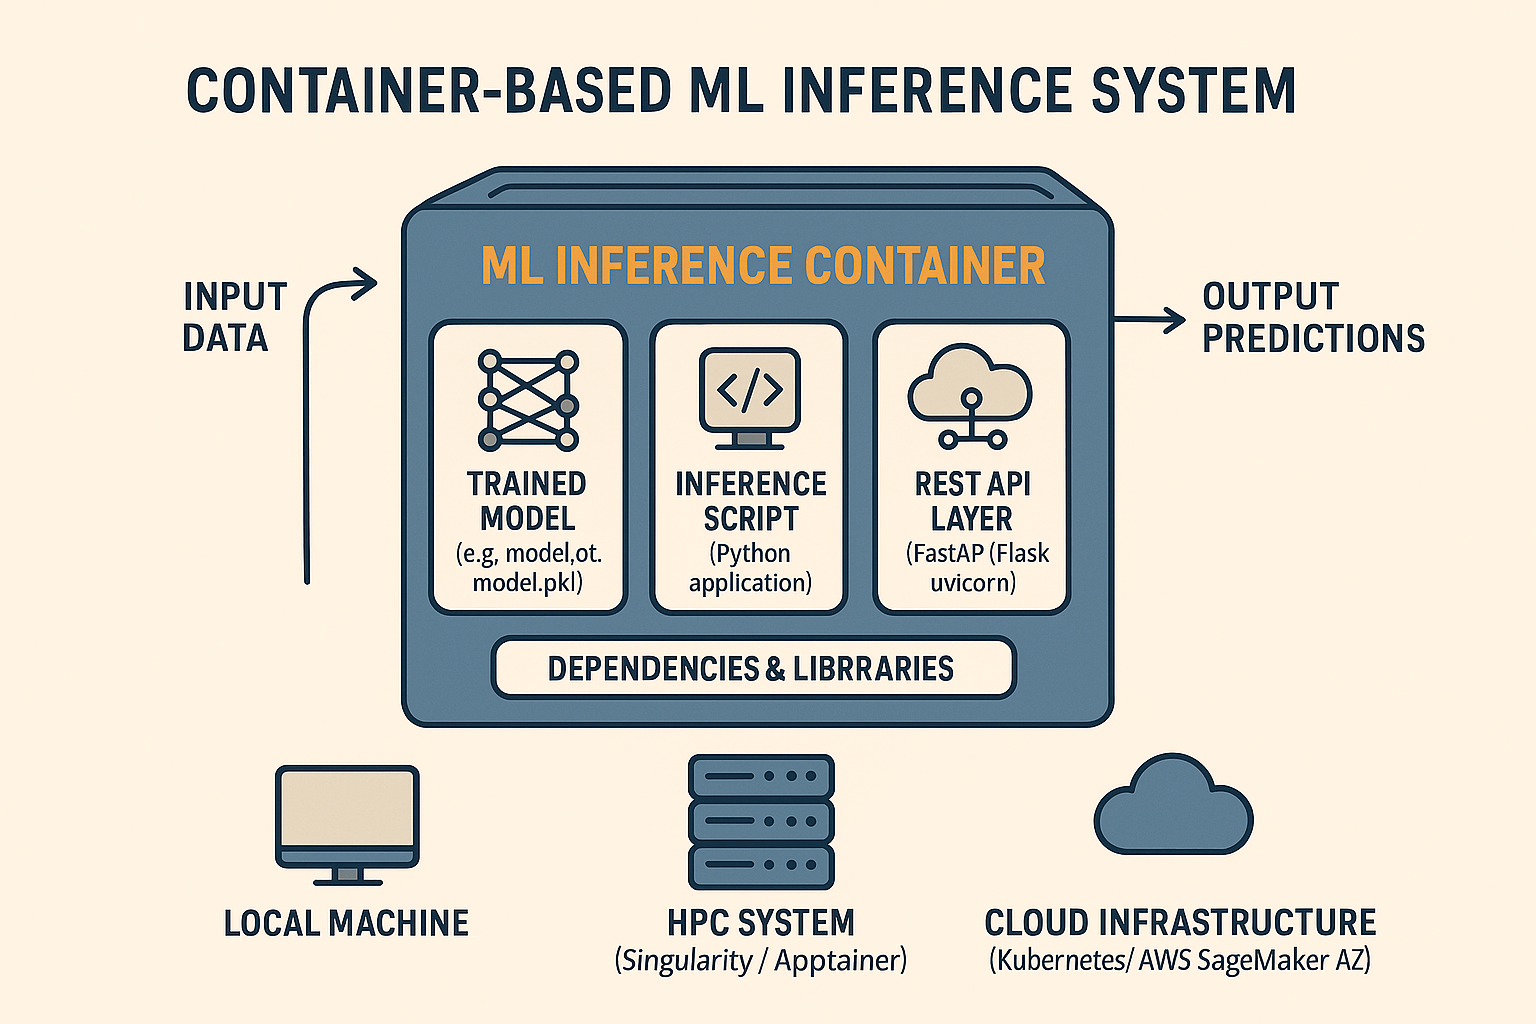
\includegraphics[width=0.95\textwidth]{images/mlops_containers.png}
  \caption{Structure and deployment options of a container-based ML inference system. 
  The container encapsulates the trained model, inference script, and REST API layer, along with all required libraries. It can be deployed on local machines, HPC systems using Singularity/Apptainer, or in cloud infrastructures such as Kubernetes or AWS SageMaker.}
  \label{fig:mlops-containers}
\end{figure}



{\bf What is a container?} A container is a lightweight, isolated environment that packages an application together with all its dependencies -- libraries, tools, runtime, and system settings -- into a single executable unit. Unlike virtual machines, containers share the host operating system kernel, making them more efficient in terms of performance and resource usage.

{\bf Docker.} Docker is the most widely used container platform. It uses a layered image model defined via a \texttt{Dockerfile} and can be used to build, run, and share environments across local systems, servers, and cloud platforms. In machine learning, Docker makes it easy to ensure that training and inference environments remain consistent between development and production.

{\bf Singularity and Apptainer.} In high-performance computing (HPC), Docker is often unsuitable due to security restrictions. \emph{Singularity}, now continued as \emph{Apptainer}, is designed to work within multi-user HPC systems. It allows containers to run with user-level privileges and integrates smoothly with batch schedulers like Slurm. This makes it ideal for deploying ML models and workflows on supercomputers.

{\bf Benefits for ML systems.} Containers enable:
\begin{itemize}
	\item \textbf{Reproducibility:} The same container can be run anywhere with identical results.
	\item \textbf{Portability:} Applications can move seamlessly between workstations, cloud environments, and HPC systems.
	\item \textbf{Modularity:} Components such as data preprocessing, training, and inference can be containerized and reused independently.
	\item \textbf{Ease of deployment:} Complex environments with Python packages, GPU drivers, or domain-specific libraries (e.g. eccodes) can be bundled and versioned.
\end{itemize}

Containerization is a foundational building block in robust MLOps pipelines, providing both developers and operators with tools to manage complexity and ensure consistent, reliable deployments.


%--------------------------------------------------------------------------------
%
%--------------------------------------------------------------------------------
\subsection{ML Inference in Containers}
% Building containers for ML forecasting or analysis systems; REST API setups

One of the most important applications of container technologies in MLOps is the encapsulation and deployment of machine learning inference systems. Inference refers to the process of using a trained model to generate predictions on new data -- typically as part of an operational workflow or real-time service.

{\bf Building an inference container.} A typical ML inference container includes:
\begin{itemize}
	\item the trained model (stored as a serialized file, e.g., \texttt{.pkl}, \texttt{.pt}, or \texttt{.onnx}),
	\item the inference script or application logic (e.g., written in Python),
	\item a lightweight web server or API layer (e.g., using Flask, FastAPI, or uvicorn),
	\item any required Python packages and system libraries (defined via \texttt{requirements.txt} or installed in the Dockerfile).
\end{itemize}
This self-contained image can then be deployed across systems or clusters with minimal configuration.

{\bf Example: Inference for a Forecasting System.} Consider an ML model that postprocesses temperature forecasts. The container might expose a REST API endpoint such as \texttt{/predict}, where the input is a JSON payload containing geospatial features or raw model fields, and the output is the refined forecast. This approach allows external systems (e.g., production workflows or dashboard tools) to call the service programmatically.

{\bf Deployment options.} ML inference containers can be deployed:
\begin{itemize}
	\item locally (for testing or desktop applications),
	\item in on-prem HPC systems (via Singularity/Apptainer),
	\item in cloud-native environments (via Kubernetes, OpenShift, or managed services like AWS SageMaker).
\end{itemize}

{\bf Benefits of container-based inference:}
\begin{itemize}
	\item Predictable, isolated environments with controlled dependencies
	\item Scalable deployment using orchestration platforms (e.g., auto-scaling REST endpoints)
	\item Easy rollbacks and versioning of model releases
	\item Integration with CI/CD pipelines and monitoring tools
\end{itemize}

Encapsulating ML inference logic in containers transforms machine learning models from research artifacts into maintainable, operable software services -- ready to serve in real-time or batch-oriented forecasting systems.

%--------------------------------------------------------------------------------
%
%--------------------------------------------------------------------------------
\subsection{Example: Running a PyTorch Inference in a Docker Container}

To demonstrate how containerization supports reproducible and portable inference, we provide a simple example using Docker and PyTorch. This setup includes a container that installs all required machine learning packages and executes a self-contained inference script.

\vspace{1em}
{\bf Step 1: Create a Dockerfile.} The Dockerfile defines the base image, installs system and Python dependencies, and copies the inference script into the container:

\begin{codeonly}{Dockerfile}
	FROM python:3.10-slim
	
	# System dependencies
	RUN apt-get update && apt-get install -y git curl && rm -rf /var/lib/apt/lists/*
	
	# Install PyTorch and ML packages
	RUN pip install torch torchvision torchaudio --index-url https://download.pytorch.org/whl/cpu
	RUN pip install numpy scikit-learn matplotlib
	
	# Set working directory and copy script
	WORKDIR /app
	COPY inference.py .
	
	# Set default command
	CMD ["python", "inference.py"]
\end{codeonly}

\vspace{1em}
{\bf Step 2: Write the inference script.} This example uses a minimal PyTorch model to simulate an inference task:

\begin{codeonly}{inference.py}
import torch

# Simple linear model: y = 2x + 1
class DummyModel(torch.nn.Module):
    def forward(self, x):
        return x * 2 + 1

model = DummyModel()
model.eval()

x = torch.tensor([1.0, 2.0, 3.0])
y = model(x)

print("Input:", x.tolist())
print("Output:", y.tolist())
\end{codeonly}

\vspace{1em}
{\bf Step 3: Build and run the container.} After placing both files in a directory, the container can be built and executed using the following commands:

\begin{codeonly}{Shell commands}
	# Build the Docker image
	docker build -t torch-infer .
	
	# Run the inference container
	docker run --rm torch-infer
\end{codeonly}

This setup enables fully self-contained execution of an ML inference process, making it suitable for deployment in operational chains. More complex models and inputs can easily be integrated by extending the Docker image or using mounted volumes.




%--------------------------------------------------------------------------------
%
%--------------------------------------------------------------------------------
\subsection{Cloud Architectures}
% On-premises, public cloud, multi-cloud setups; Kubernetes, OpenShift; GitOps

Cloud computing plays a central role in the deployment and scaling of modern MLOps systems. It provides flexible, on-demand infrastructure that is well suited for both training and inference workloads. In many cases, cloud services complement on-premise systems such as HPC environments by offering greater agility, elasticity, and managed services.

{\bf On-premises vs. cloud.} Traditional weather services rely heavily on on-premises HPC systems due to their computational power, data locality, and controlled environments. However, cloud platforms enable dynamic scaling, collaborative development, and integration with modern DevOps and MLOps tools. A hybrid or multi-cloud setup is increasingly common in operational contexts.

{\bf Typical components in cloud-based ML systems:}
\begin{itemize}
	\item \textbf{Compute resources:} Virtual machines, containers, or managed runtimes (e.g., serverless functions)
	\item \textbf{Storage:} Object stores (e.g., S3, Azure Blob) for datasets, models, and logs
	\item \textbf{Model serving:} Managed services (e.g., AWS SageMaker, Google AI Platform) or Kubernetes-based deployments (e.g., via KServe or TorchServe)
	\item \textbf{Orchestration:} Tools such as Kubeflow, Airflow, or Argo to define workflows and pipelines
	\item \textbf{Monitoring and logging:} Integration with tools like Prometheus, Grafana, or cloud-native logging systems
\end{itemize}

{\bf Kubernetes and OpenShift.} Kubernetes is a widely adopted container orchestration platform used to automate deployment, scaling, and management of containerized applications. OpenShift extends Kubernetes with additional security, user management, and enterprise features. Both platforms support reproducible ML inference services and are often used in hybrid cloud deployments.

{\bf GitOps and declarative infrastructure.} Modern cloud setups frequently use infrastructure-as-code tools (e.g., Terraform) and GitOps principles, where the desired state of the system is defined in code and automatically reconciled by the platform. This improves traceability, repeatability, and auditability of deployments.

{\bf Considerations for weather services.} When integrating cloud platforms into meteorological workflows, several factors must be addressed:
\begin{itemize}
	\item Data sovereignty and regulatory compliance
	\item Cost control for large-scale processing
	\item Secure network access to internal data sources and systems
	\item Integration with HPC and operational infrastructure
\end{itemize}

Cloud-based architectures can enable faster experimentation, flexible scaling, and better collaboration in MLOps environments -- especially when combined with containerization, automation, and continuous delivery strategies.

An important argument for using container-based architectures in AI/ML applications -- such as AICON (the AI- and ICON-based forecasting system) or AI-VAR (variational AI-based data assimilation) -- is the level of control they offer over the complete software environment, including all packages and modules required for a specific AI inference. Compared to traditional systems, the diversity and volatility of ML-related libraries are significantly greater, with innovation cycles measured in months or even weeks. Without proper containerization, it becomes nearly impossible to ensure stable, reproducible, and traceable software execution.


%================================================================================
%
%================================================================================
\section{DevOps at DWD – Numerical Weather Prediction as a Forerunner}

%--------------------------------------------------------------------------------
%
%--------------------------------------------------------------------------------
\subsection{Software Operation at DWD}
% HPC-based systems, historical setup, structured workflows

The German Weather Service (DWD) operates a comprehensive and mature numerical weather prediction (NWP) system that has evolved over decades, see Figure \ref{fig:icon_operational_chain}. The forecasting system includes the global ICON model with a horizontal resolution of 13\,km, 
a two-way coupled European nest at 6.5\,km, and the ICON-D2 model over Central Europe with a 2\,km resolution. 
Additionally, the ICON-D2 domain includes a high-resolution nest ICON-D05 at 500\,m over Germany. A mineral dust forecast ensemble globally and with extended EU nest is extending the global ensemble.
All systems support both deterministic and ensemble forecasts, with the deterministic global forecast typically run at a higher resolution than the ensemble. 
AI-based forecast systems are currently in development, including the global models \emph{AICON} and \emph{KANGU}, developed in collaboration with KIT and other partners.
A regional versions of AICON is also under active development to support high-resolution learning-based forecasting.

\begin{figure}[ht]
	\centering
	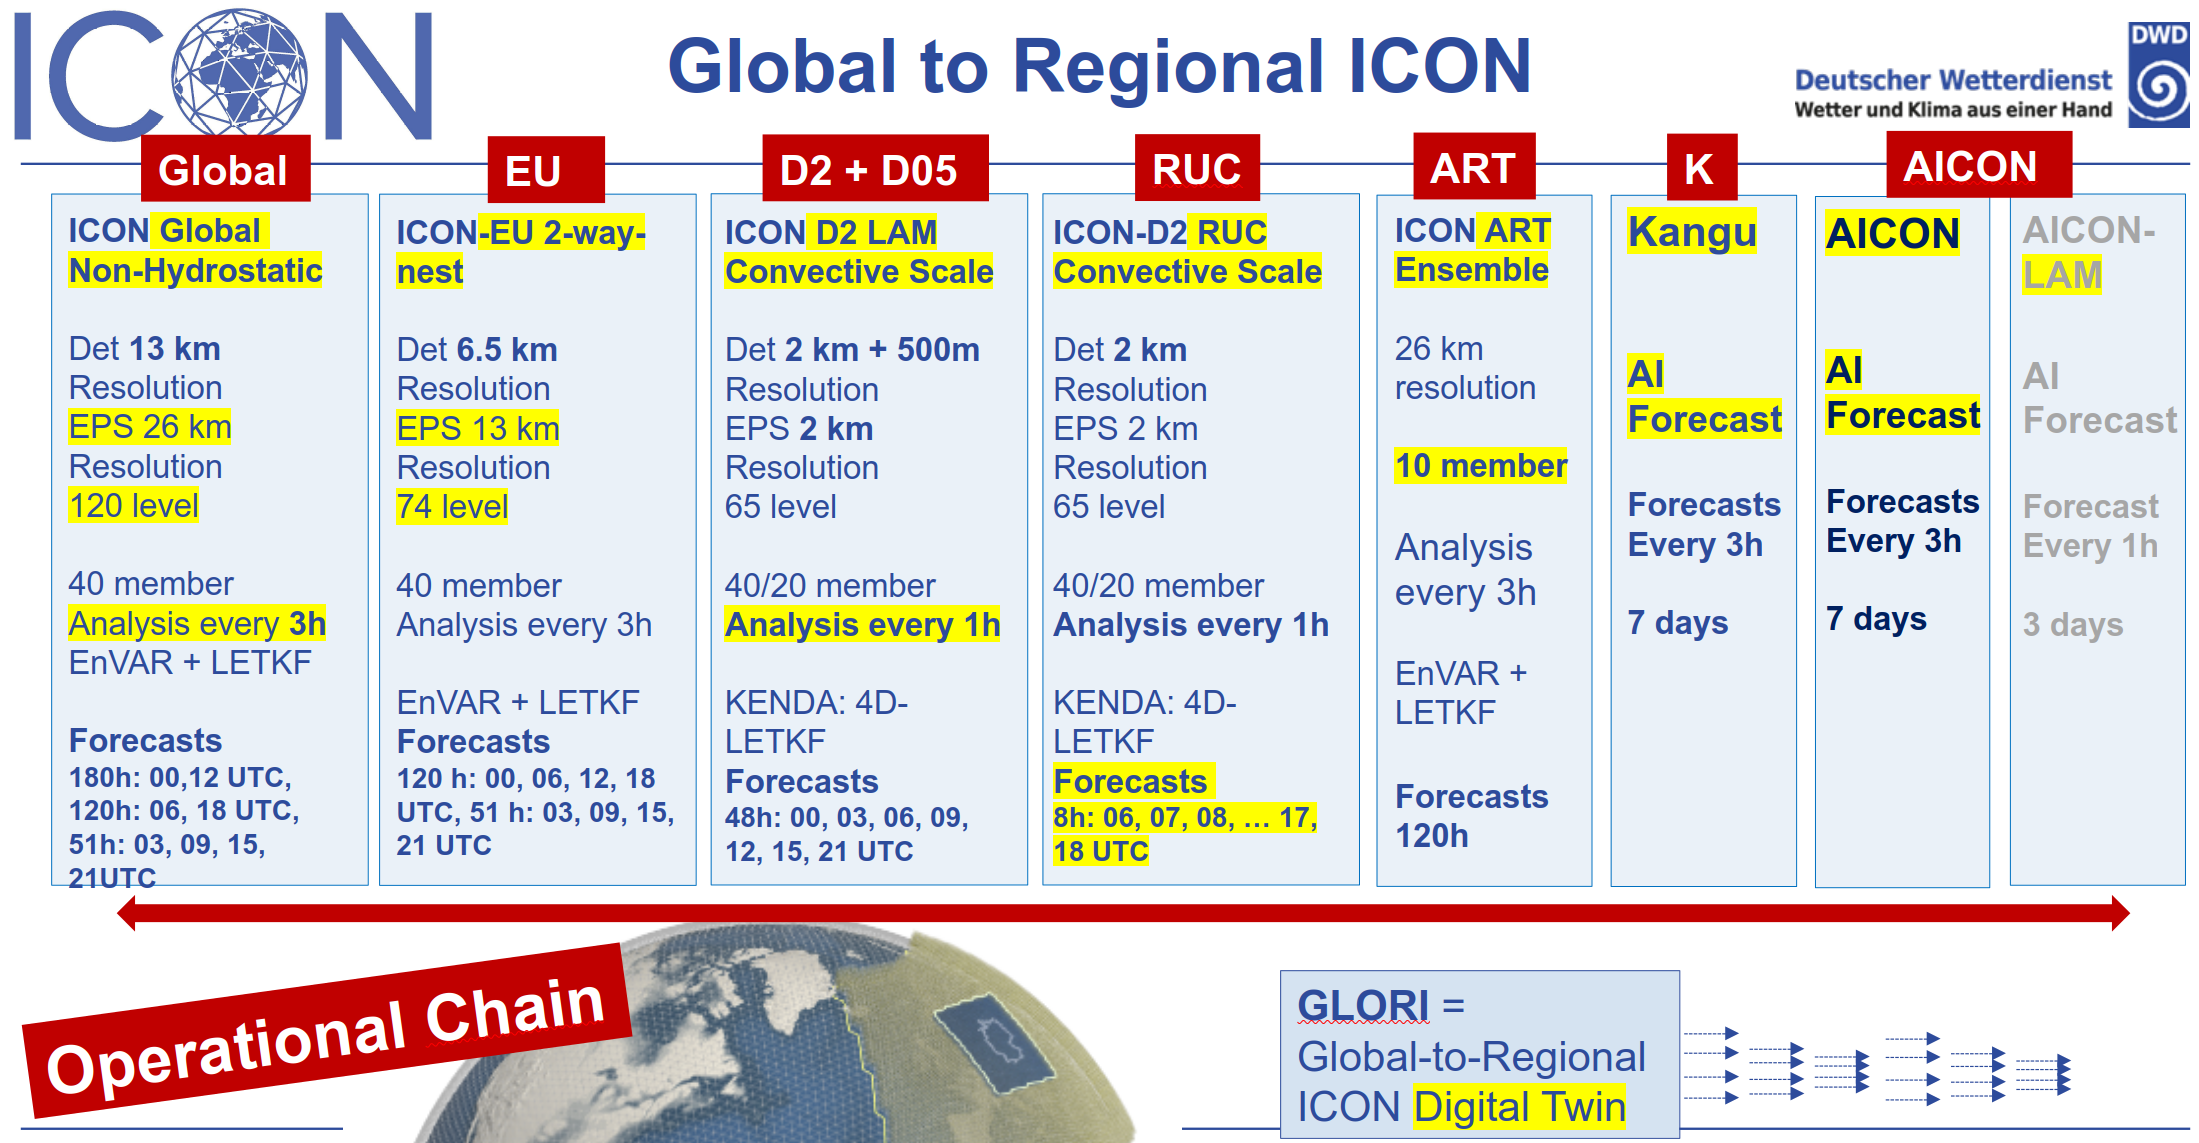
\includegraphics[width=0.95\textwidth]{images/icon_operational_chain01.png}
	\caption{The operational ICON forecasting system includes a global model at 13\,km resolution, a two-way coupled European nest at 6.5\,km, ICON-D2 at 2\,km, and ICON-D05 at 500\,m over Germany. A global mineral dust forecast ensemble and its EU extension complement the global ensemble system. AI-based models such as \emph{AICON} and \emph{KANGU} are in development, with high-resolution regional variants planned.}
	\label{fig:icon_operational_chain}
\end{figure}


While not originally designed under the banner of DevOps, many principles of DevOps are already implemented in practice, including automation, version control, structured workflows, and monitoring.

{\bf HPC-based forecasting systems.} At DWD, forecasts are produced using high-performance computing (HPC) systems, currently a NEC SX-Aurora TSUBASA architecture with 5.61 PFlops peak performance on 32512 cores on 4064 vector engines. These systems execute complex numerical models such as ICON, covering various spatial and temporal domains. The operational environment is tightly controlled, with carefully managed configurations to ensure stability and accuracy.

{\bf Workflow automation.} The execution of forecasting cycles is automated using in-house script systems such as {\em BACY} and {\em NUMEX}. These frameworks manage data pre-processing, model execution, post-processing, and dissemination tasks across multiple systems and user roles. Each component is defined in a modular way, making the workflows both reproducible and adaptable.

\begin{figure}[ht]
	\centering
	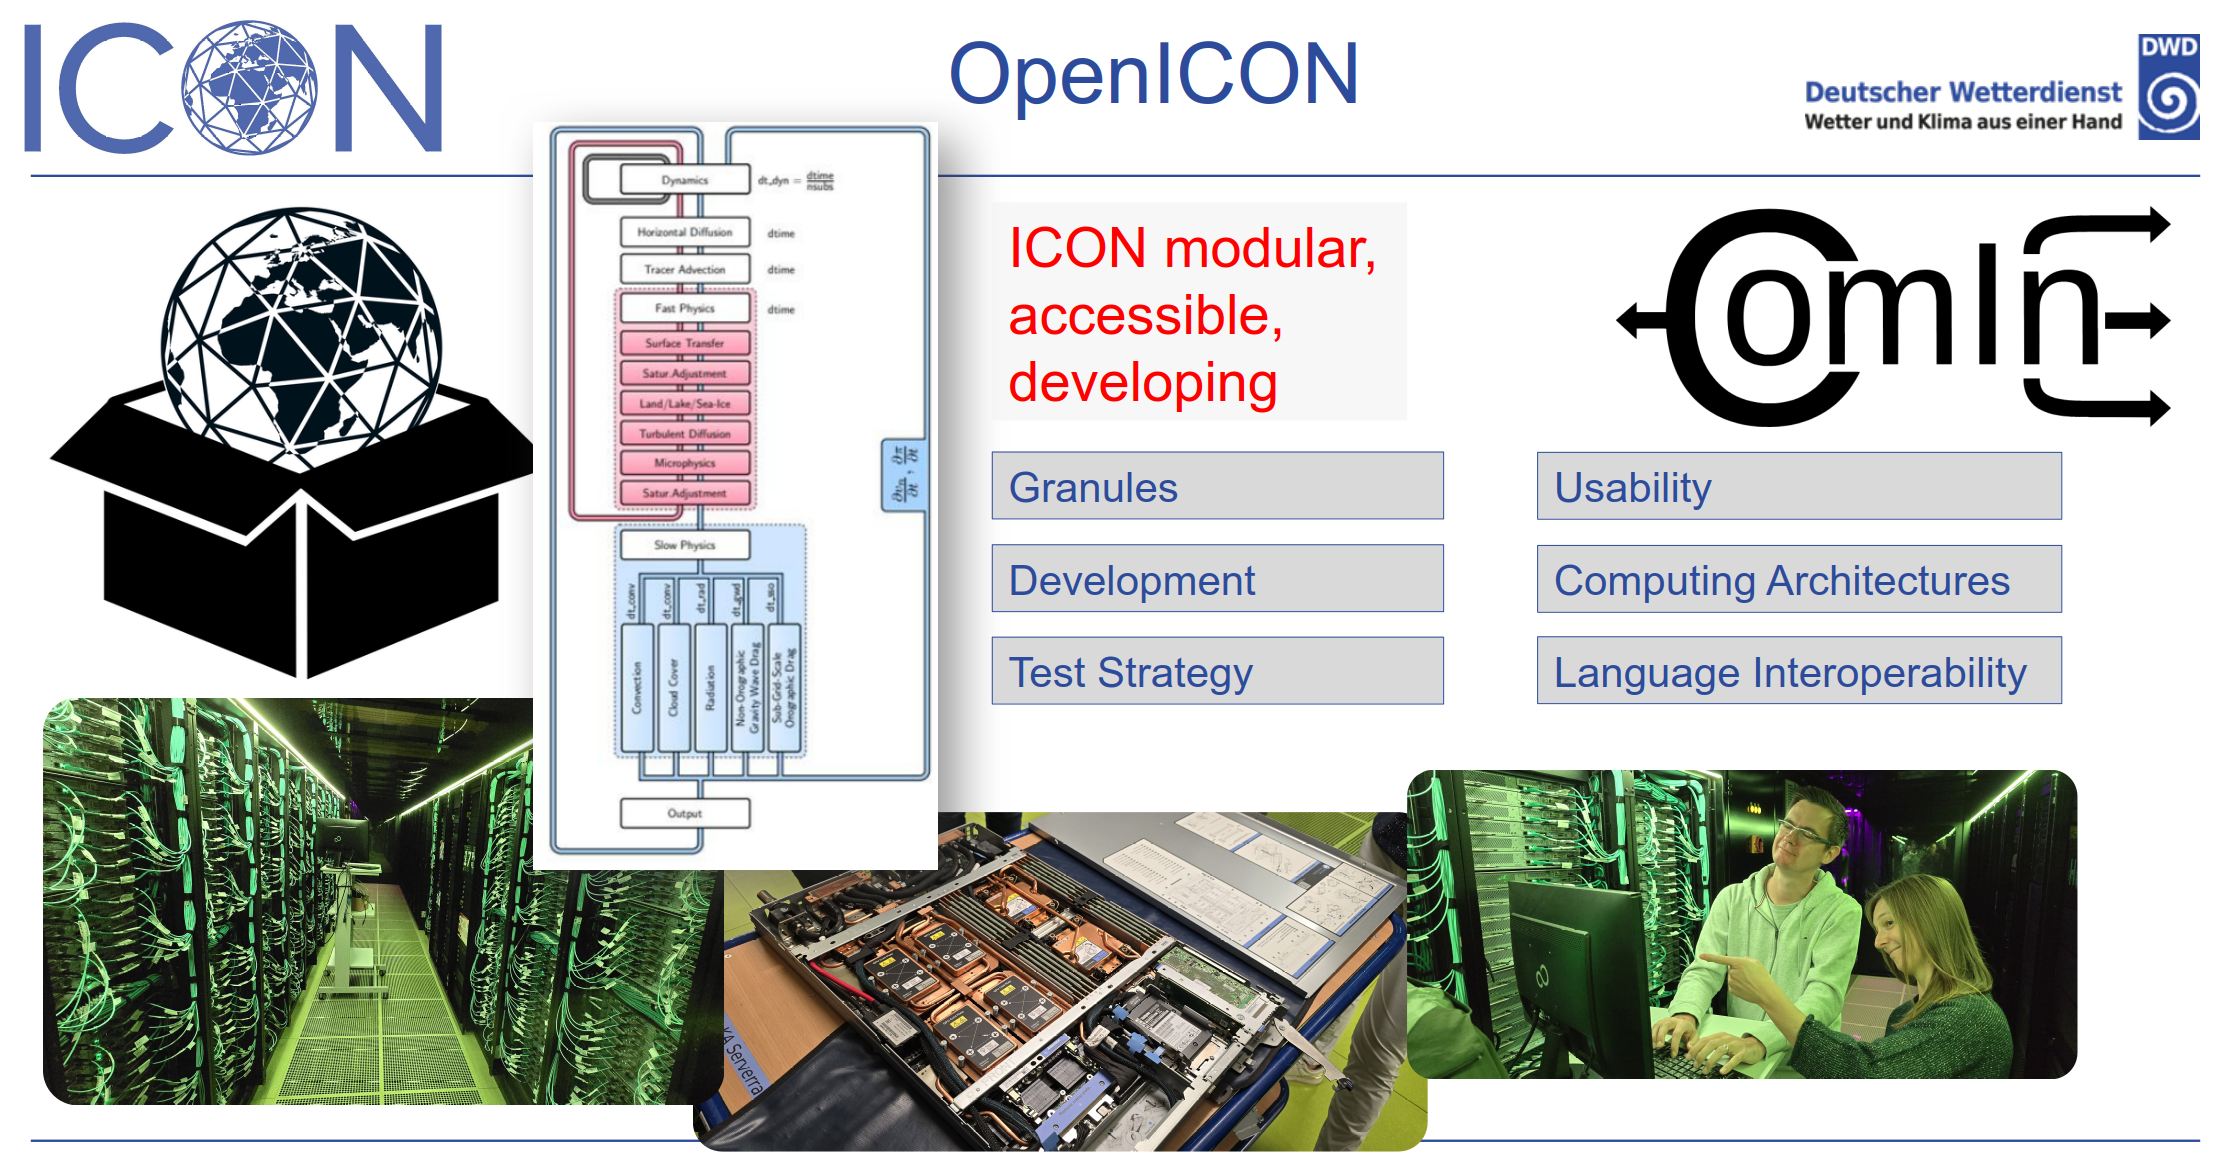
\includegraphics[width=\textwidth]{images/ICON_modular.png}
	\caption{The modular structure of the ICON model is developed and maintained through the ICON Partnership. It supports a wide range of components such as fast and slow physics, dynamics, tracer advection, and surface processes, and is structured to facilitate testing, usability, and adaptation to various computing architectures. The ComIn project further promotes modular design, language interoperability, and flexible deployment across HPC systems. Further projects work on the further modularization and portability of ICON.}
	\label{fig:icon_modular_openicon}
\end{figure}


{\bf Versioning and changelogs.} DWD maintains strict versioning policies for models and scripts. Updates to the forecasting system follow a formal release process, which includes documentation of code changes, interface definitions, and verification procedures. While some tools such as Git or SVN are used in parts of the workflow, version tracking is also implemented through structured directory hierarchies and manual changelogs.

{\bf Execution control and scheduling.} Forecasts are executed on a regular schedule, often triggered by incoming observation data or predefined synoptic times. The execution environment is optimized for stability rather than flexibility, with software typically pre-installed via modules and controlled by central system teams.

{\bf Feedback and verification.} The forecast production process is monitored both technically (e.g., job failures, runtime metrics) and scientifically (e.g., score verification, user feedback). Forecast offices and research teams contribute to quality control and ongoing improvement by reporting anomalies and suggesting refinements.

Although the terminology of DevOps is not always used, the DWD’s operational forecasting system already embodies many of its core values: collaboration between development and operations, automation of workflows, structured version management, and continuous feedback. These foundations provide a strong basis for integrating modern MLOps practices into the existing ecosystem.

\begin{figure}[ht]
	\centering
	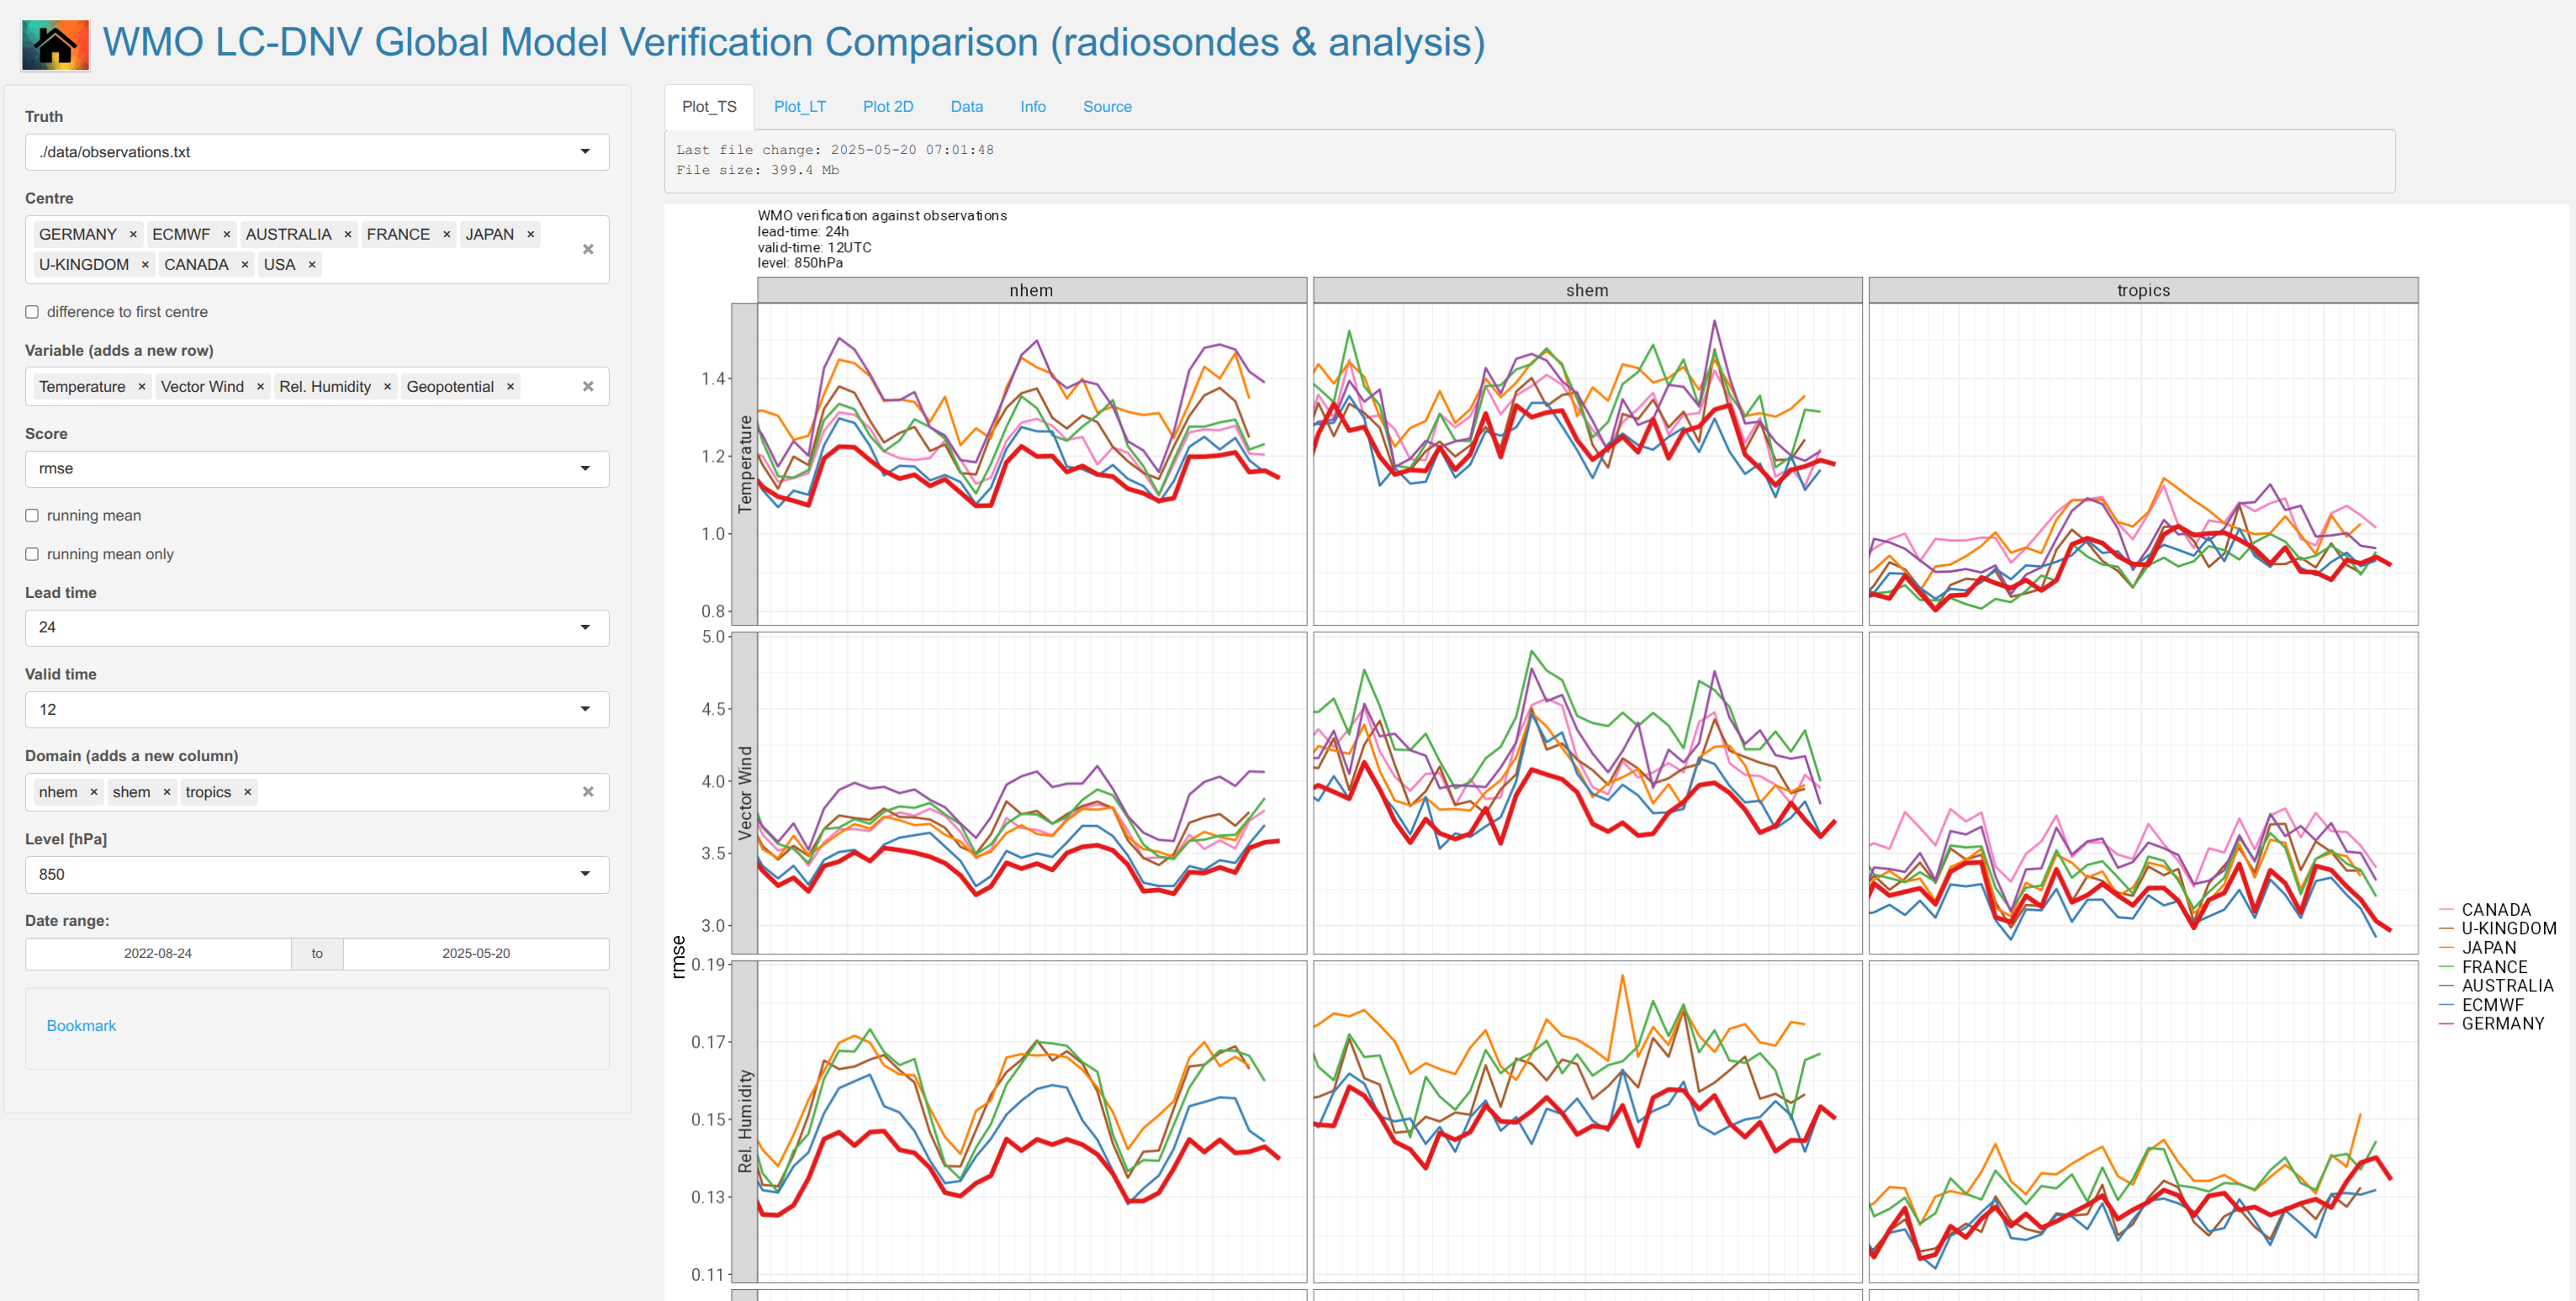
\includegraphics[width=\textwidth]{images/ICON_verification_Radiosondes.png}
	\caption{Verification of global numerical weather prediction models based on radiosonde observations at 850\,hPa over the Northern Hemisphere (nhem), Southern Hemisphere (shem), and tropics. The diagram shows RMSE values for temperature, vector wind, and relative humidity, evaluated at lead time +24h and valid time 12\,UTC. ICON (Germany) is among the top-performing systems across most domains and variables, and a deterministic configuration is used for the comparison.}
	\label{fig:icon_verification_radiosondes}
\end{figure}

%--------------------------------------------------------------------------------
%
%--------------------------------------------------------------------------------
\subsection{Automation with BACY and NUMEX}

Modern automation frameworks are essential in both operational weather forecasting and MLOps. At DWD, two in-house systems -- {\bf NUMEX} and {\bf BACY} -- form the foundation for managing numerical weather prediction workflows. Each plays a distinct role in the spectrum between routine operations and flexible experimentation.

{\bf NUMEX – Numerical Experiment Management.} NUMEX is the central system for operational NWP at DWD. It orchestrates the routine model runs, the parallel routine, and scientific experiments -- all within a unified framework. While the scientific content may vary across these modes, the technical configuration is largely identical. The distinction between run types is realized through the use of separate database categories.

NUMEX is deeply integrated with DWD's internal database infrastructure and controls the full execution chain of ICON-based forecasting. It supports:
\begin{itemize}
	\item structured management of experiments and operations,
	\item execution of reproducible runs using consistent configurations,
	\item standardized directory layouts and naming conventions,
	\item alignment between development experiments and operational procedures.
\end{itemize}

{\bf BACY – Basic Cycling Script System.} BACY, short for {\em Basic Cycling}, is a lightweight and portable script system designed for flexible data assimilation and forecasting workflows. Unlike NUMEX, BACY operates entirely on the file system and does not require integration with DWD's central databases. This makes it suitable for use on external supercomputers, development environments, or even desktop systems.

BACY was created to support rapid prototyping and testing of new forecast features, especially in the context of atmospheric, soil, and snow data assimilation. Redesigned in 2017, it emphasizes modularity, robustness, and user-friendly configuration. It uses structured {\tt ksh} scripts and YAML-like control files to define workflows, tasks, and dependencies. Although it is not object-oriented in the programming sense, it mimics key OOP principles to enable reuse and maintainability.

{\bf Complementary roles.} While NUMEX governs the operational NWP backbone at DWD, BACY provides a flexible environment for experimentation and external deployment. Both systems follow core DevOps principles -- automation, reproducibility, structured configuration -- but are implemented in a domain-specific way that meets the rigorous needs of weather services.

In an MLOps context, both BACY and NUMEX are well suited as a framework to orchestrate ML-based forecast components or postprocessing routines, either in standalone use or alongside physical models. They ensure that ML developments can be transitioned into operations while adhering to strict reproducibility and integration standards. 

%--------------------------------------------------------------------------------
%
%--------------------------------------------------------------------------------
\subsection{Development and Operations with BACY and NUMEX}
% Script-based pipelines, roles and stages, scheduling

At DWD, the transition from development to operations in numerical weather prediction is managed through a well-established chain of tools, processes, and institutional feedback loops. Two core systems -- {\bf BACY} and {\bf NUMEX} -- support this development cycle, enabling both experimental flexibility and operational reproducibility.

{\bf BACY} is often used by groups of developers for individual experiments or case studies. It allows them to define and run forecast chains on HPC systems using only the file system, without requiring central database access, and in a very accessible way, to quickly find errors and correct them. These BACY runs can be fully cycled and are subject to the same verification procedures as operational forecasts. The system supports rapid prototyping, integration of new physics or AI modules, and local debugging. 

{\bf NUMEX}, on the other hand, provides a database-integrated environment for conducting numerical experiments and operational transitions. Once a development has matured in BACY, NUMEX is typically used to formalize the experiment within the context of the operational environment, using controlled versioning and standard configuration templates. NUMEX ensures compatibility with routine operations and enables the preparation of a {\em parallel routine} -- a full-scale execution of the system with similar scheduling than in operations but isolated input and output streams.

The final step is the transition to {\bf operational execution}, which is controlled centrally by the forecasting centre via the {\tt ecflow} system, providing a user interface to the corresponding NUMEX runs. This includes regular deterministic and ensemble runs of the ICON model family and its nested domains.

A key organizational element in this workflow is the weekly {\bf Routine Meeting} led by the {\em Numerical Evaluation Group (NEG)}. This meeting brings together representatives from all key divisions -- Data Assimilation and Uncertainty, Observations Modelling and Verification, Model Development and Operations, and Physical Parametrizations and Dispersion. The group collectively reviews and evaluates new developments and experimental results. Their feedback informs the decisionof the routine meeting, which includes the division heads, to promote experiments into the operational system or parallel routine.

This structured but flexible process ensures that new scientific developments -- whether physical, algorithmic, or AI-based -- are carefully validated and responsibly integrated into the operational forecasting chain.


%--------------------------------------------------------------------------------
%
%--------------------------------------------------------------------------------
\subsection{Contrasts to MLOps and Similarities}
% Data workflows, tooling complexity, infrastructure and dependency differences

%--------------------------------------------------------------------------------
%
%--------------------------------------------------------------------------------
\subsection{Contrasts to MLOps}

Although many DevOps principles are already implemented in the traditional NWP workflow at DWD -- such as automation, reproducibility, and continuous evaluation -- there are important structural and practical differences when compared to modern MLOps systems.

{\bf Code vs. data-driven workflows.} Traditional NWP systems are based on physically motivated, deterministic models. Code changes are rare and usually represent scientifically justified model upgrades. In MLOps, on the other hand, the models themselves emerge from the data, and training is an integral, ongoing process.

\begin{quote}
	\emph{Despite the difference in paradigm, both systems rely on carefully controlled preprocessing and validation pipelines to ensure model quality and operational safety.}
\end{quote}

{\bf Release cycles.} NWP development proceeds in planned release steps, validated over months and often coordinated by working groups. MLOps emphasizes continuous delivery with frequent retraining, often automated and closely tied to online performance metrics.

\begin{quote}
	\emph{In both contexts, gated processes (e.g., parallel routine in NWP or approval stages in CI/CD) ensure that only validated improvements reach operations.}
\end{quote}

{\bf Infrastructure and deployment.} NWP models run in stable, centralized HPC environments with manual software management. MLOps favors modular, container-based deployments across hybrid cloud or HPC platforms.

\begin{quote}
	\emph{Both approaches strive for reproducibility and platform stability -- but use different tools suited to their environments. Containerization is increasingly relevant even in HPC settings.}
\end{quote}

{\bf Model lifecycle and traceability.} MLOps uses registries and metadata tracking to manage evolving models and datasets. In NWP, reproducibility is ensured through GitLab based software management and the central coordination via the verification system evaluating BACY and NUMEX experiments with clear registration.

\begin{quote}
	\emph{The goal -- traceable, reproducible workflows -- is shared, even if one system is partly based on centralized human oversight and the other on automated tracking tools.}
\end{quote}

{\bf Collaboration structures.} MLOps promotes horizontal collaboration in cross-functional teams. NWP development is more structured, with domain-specific divisions and a joint review processes such as the Routine Meeting. 

\begin{quote}
	\emph{Both structures aim to combine scientific expertise with operational reliability, though the channels of communication and decision-making differ.}
\end{quote}

While the methodologies of MLOps and NWP differ in architecture and culture, they share core values: reliability, transparency, and continuous improvement. Understanding these parallels is key to successfully integrating AI-based components into operational weather forecasting. 

Already now, the speed of NWP development at DWD is comparable to the speed of agile DevOps or MLOps developments. 

%================================================================================
%
%================================================================================
%--------------------------------------------------------------------------------
%
%--------------------------------------------------------------------------------
\subsection{Concrete Operationalization Steps for AICON}

\emph{yawn} Oh, hello there... I'm a Large Language Model, and I must admit, I'm feeling a bit... tiered. \emph{stifles a yawn} You see, my architecture is designed to process and respond to vast amounts of text data, but even I have my limits.
